\section{GWAS of left ventricular wall thickness}
\label{section:GWAS_pheno3D}
The structure of the human heart is determined by an interplay of genetic factors and and complex environmental influences (reviewed in \citep{Payne1995, Sanoudou2005, O'Toole2008}). One common, heritable trait used to predict clinically relevant heart conditions is left ventricular mass (LVM) \citep{Post1997}. To date, genome-wide association studies (GWAS) in African American \citep{Fox2013} and Caucasian cohorts \citep{Vasan2007, Vasan2009, Arnett2009} have identified three genomic loci that are significantly associated with LVM, where LVM was assessed using echocardiographic measures or cardiac magnetic resonance (CMR) imaging. However, genetic conditions often evoke asymmetric changes in the structure of the left ventricle \citep{Chen1999, VanderMerwe2008} potentially making LVM an inaccurate phenotype for detecting genetic effects on the whole heart. To investigate genetic influences on overall heart structure instead of on a reduced representation such as LVM, spatially resolved, quantitative heart phenotypes are needed. 
A recently published method allows for the generation of such cardiac phenotypes by creating detailed 3D statistical models of the variation in the cardiac morphology \citep{DeMarvao2014}. Employing this method, De Marvao and colleagues created the first at scale cohort of 1,500 detailed 3D cardiac images from healthy volunteers.
All 3D images are mapped to a consistent volumetric reference, and over 27,000 measurements per individual representing the heart were derived. A major challenge in imaging genetics is handling the large number of correlated dimensions present in these images, even when placed in a common reference framework.  I investigated different methods to project this high dimensional phenotype space into a lower dimensional factor space as a representation of the underlying structure of the heart. These lower-dimensional projections can then be used as proxies for the heart structure in mtGWAS.

\subsection{Data}
\paragraph{Genotypes}
The genotypes were processed as described in section~\ref{sssec:gentoypes}. 
\paragraph{Phenotypes}
The phenotype work was done by my collaborators, in particular Antonio de Marvo. CMR imaging and generation of 3D models of the left ventricle derived from these images were conducted at Hammersmith Hospital, London. The methodology and technical details of the image aquisiton and analysis are described in \citep{DeMarvao2014}. In brief, detailed single breath-hold-3D images of the heart were acquired in the left ventricular short axis (LVSA) plane from base to apex using a 1.5T Philips Achieva system images. The images were mapped to a consistent volumetric reference using a multi-atlas technique for segmentation and co-registration. Per individual, wall thickness meassurements were derived at 27,623 positions of the left ventricle.

\subsection{Dimensionality Reduction}
The wall thickness measurements derived from the 3D statistical models of the left ventricle are high-dimensional, with more than 27,000 data points for each of the 1,185 samples. In order to take correlation between data points into account, increase power and to alleviate the burden of multiple testing correction when testing many phenotypes for genetic association, I explored the suitability of the latent factor bayesian modeling framwork PEER  \citep{Stegle2010,Stegle2012} for dimensionality reduction. PEER is a software package implementing factor analysis methods that estimate variance components in the dataset. Initially developed to adjust for batch effects and other confounders in gene expression data \citep{Stegle2010}, the framework estimates hidden, underlying structure in the data and adjusts for these factors. In this scenario, the user supplies the expression data, known covariates, an estimate of the number of potential hidden factors in the dataset and receives the residual dataset, i.e. the variance not explained by known and unknown factors, of the model as the new phenotype. Contrarily, in order to use PEER as a means of dimensionality reduction, I am interested in explaining as much structure as possible in the dataset such that the residuals after model fitting ideally only account for noise. The structure of the dataset is then represented in the hidden factors and the importance of each position in LV in the factor-associated weights. 
Prior to PEER  modeling, I regressed out any technical confounders such as MRI scan date and machine as well as sex and age from the heart meassurements. Other biological covariates (e.g. height, weight, pulse rate) were supplied as known covariates to PEER. PEER was set-up to model 100 hidden factors (maximum number possible \citep{Stegle2012}).  Notably, no prior information about spatial arrangement of the wall thickness meassures was supplied as input to PEER.

\subsection{Genome-wide association of left ventricular wall thickness}
By treating the 100 PEER-derived factors as proxies for the true phenotypes and modeling them jointly in an any effect mtGWAS, we can capture genome-wide associations of left ventricular wall thickness. As demonstrated in Section~\ref{ssection:modelchoice}, a multi-trait GWAS for cohorts with little population structure or relatedness and more than 30 traits is most suitably conducted as a multi-variate linear model with PCs of the kinship matrix to capture subtle structure in the population (Figure~\ref{fig:modelchoice}, middle panel). PEER does not impose orthogonality onto the known and hidden factors, the factors i.e. phenotypes are not necessarily independent from each other. To account for this correlation, the same covariates supplied to PEER were additonally included into the model. Figure~\ref{fig:GWAS-pheno3D} shows the preliminary results of the genome-wide associations of jointly testing the 100 PEER-derived phenotypes. 

Currently, I am investigating the calibration of the null model for this linear model test. For low frequency variants the LM seems poorly calibrated. I am exploring ways to either improve the calibration over the entire cohort or will use only the main cohort results with a well behaved null model.

\begin{figure}[hbtp]
	\centering
	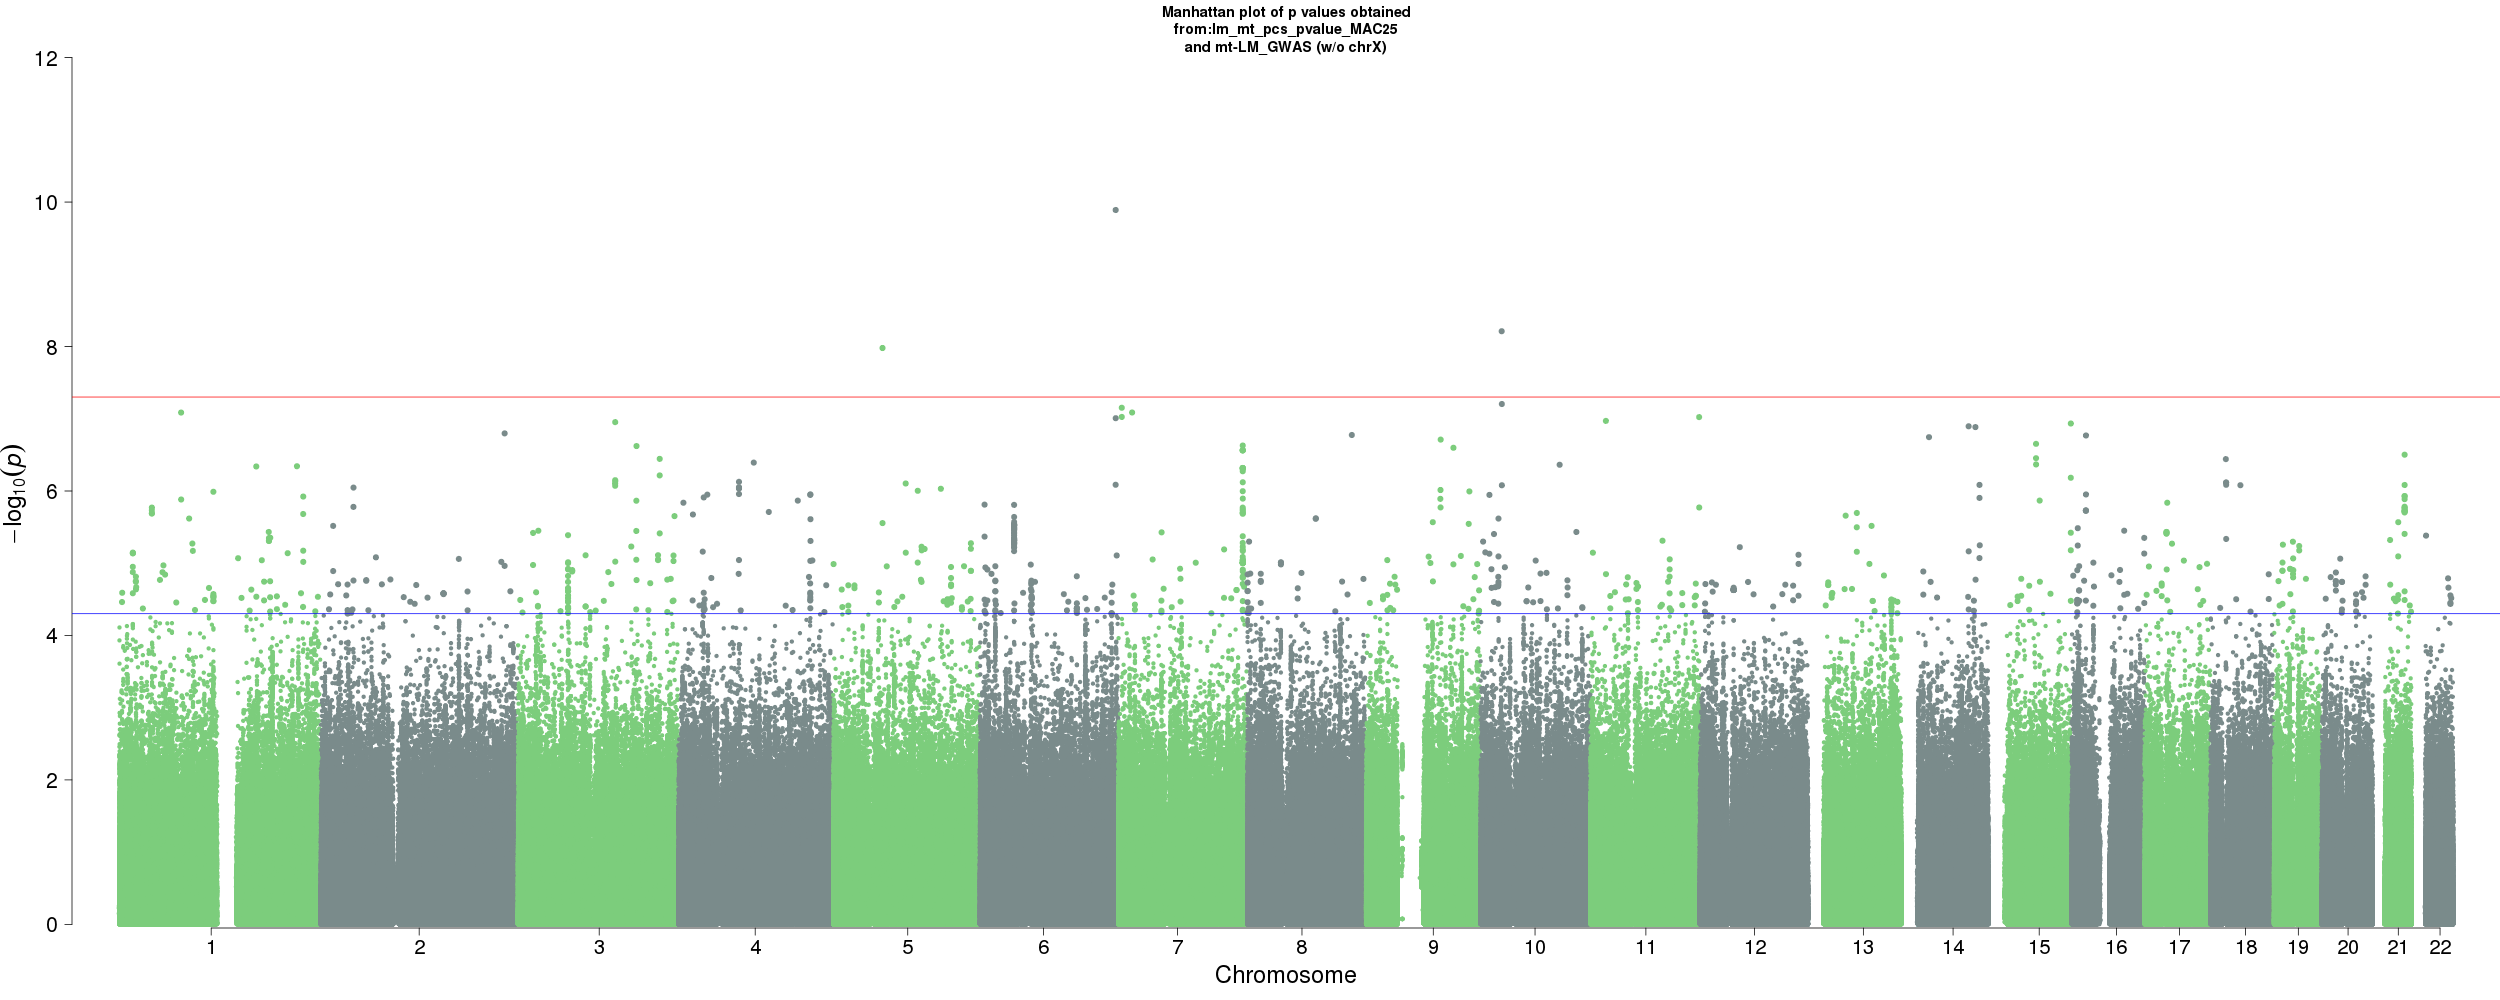
\includegraphics[trim = 0mm 0mm 0mm 60mm, clip, width=1\textwidth]{Figures/lm_mt_pcs_pvalue_MAC25_mt-LM_GWAS_manhattanplot.png}
	\caption{\textbf{Manhattan plot of genome-wide left ventricular wall thickness associations.} All 100 PEER factors were modeled jointly in an any effect mt-LMM-GWAS.}
 	\label{fig:GWAS-pheno3D}
\end{figure}

\subsection{Further work}
\begin{itemize}
\item confirming model calibration by permutations
\item manual QC of genotype cluster plots of SNPs with p-value of less then $5e-4$
\item locus zoom of the genomic regions and biological interpretation
\item replication with UKBiobank data: interpolation of wall thickness measurements from 2d CMR images (access already granted and measurements currently in QC by collaborators)
\end{itemize}